\documentclass[../problems.tex]{subfiles}

\graphicspath{{../images/}}

\begin{document}
\section{Energy}
\barh

\paragraph{4.2}
From the origin $O$ to point $P = (1,1)$ a two dimensional force $\vb{F} = (x^2, 2xy)$ 
moves a point along three paths where the work done by the force is 
\begin{equation*}
    W = \int_O^P \vb{F} \cdot \dd{\vb{r}} = \int_O^P F_x \dd{x} + F_y \dd{y}
\end{equation*}
(a) Splitting the path into two parts $O \to Q=(1,0)$ and $Q \to P$, we have two integrals
\begin{align*}
    W &= \int_O^Q F_x \dd{x} + \int_Q^P F_y \dd{y}
\end{align*}
where the first integral accounts for just the $x$ component of force $F_x = x^2$ and the second
integral accounts for just the $y$ component of force when $x=1$; $F_y = 2(1)y$. Thus
\begin{align*}
    W = \int_0^1 x^2 \dd{x} + \int_0^1 2y \dd{y} = \frac{4}{3}
\end{align*}

(b) The path follows the parabola $y=x^2$ from $O \to P$. From $\dd{y} = 2x \dd{x}$ the integral
can be rewritten in terms of just $x$
\begin{align*}
    W = \int_0^1 x^2 \dd{x} + \int_0^1 2x (x^2) \dd{y} 
    = \frac{1}{3} + \int_0^1 4x^4 \dd{x} = \frac{17}{15}
\end{align*}

(c) Path follows the parametric curve $x=t^3$ and $y=t^2$ where the differentials are:
$dx = 3t^2 \dd{t}$ and $dy = 2t \dd{t}$. Thus the work done on the path is
\begin{align*}
    W = \int_0^1 (t^6) (3t^2 \dd{t}) + \int_0^1 (2t^3) (2t \dd{t}) 
    = \frac{1}{3} + \frac{4}{5} = \frac{19}{15}
\end{align*}

\paragraph{4.3}
Same as Problem 4.2 but with a force $\vb{F} = (-y,x)$ and three different paths from $P = (1,0) \to
Q = (0,1)$.

(a) This path follows a straight line $y = 0$ from $P \to O$ and then $x = 0$ from $O \to Q$. Thus 
the work done is 
\begin{align*}
    W = \int_P^O F_x \dd{x} + \int_O^Q F_y \dd{y} = 0
\end{align*}

(b) A straight line from $P \to Q$ is given by $y = -x + 1$ and the differential $dy = -dx$. Thus
the work done is
\begin{align*}
    W = \int_P^Q F_x \dd{x} + F_y \dd{y} 
    = \int_1^0 (-(-x+1)) \dd{x} + (x) (-\dd{x}) = \int_1^0 -1 \dd{x} = 1
\end{align*}

(c) The path of a quarter circle centered on the origin in polar coordinates is given by
\begin{align*}
    x = r \cos \phi \qquad y = r \sin \phi
\end{align*}
where $r=1$, $\phi = 0 \to \pi/2$ and the differentials are
\begin{align*}
    dx = \cos \phi d{r} - r \sin \phi \dd{\phi} = - \sin \phi \dd{\phi} \qquad
    dy = \sin \phi d{r} + r \cos \phi \dd{\phi} = \cos \phi \dd{\phi}
\end{align*}
Thus the work done is
\begin{align*}
    W = \int_P^Q F_x \dd{x} + F_y \dd{y} 
    = \int_0^{\pi/2} (-\sin \phi) (-\sin \phi \dd{\phi}) + (\cos \phi) (\cos \phi \dd{\phi})
    = \int_0^{\pi/2} \dd\phi = \frac{\pi}{2}
\end{align*}

\paragraph{4.5}
(a) Given the force of gravity $\vb{F} = -mg \vu{y}$ and vertical height from 1 to 2 $h = y_2 - y_1$
, the work done by gravity is 
\begin{align*}
    W_{g}(1 \to 2) = \int_1^2 \vb{F} \cdot \dd{r} = \int_0^h -mg \dd{y} = -mgh
\end{align*}
Since the force $\vb{F}$ depends only on position and the work done by is independent of the path
taken, the force is conservative.

(b) The gravitational potential energy of the particle is 
\begin{align*}
    U_g(\vb{r}) = - W_g(0 \to \vb{r}) = - \int_0^{\vb{r}} \vb{F} \cdot \dd{\vb{r}} 
    = - \int_0^{\vb{r}} -mg \dd{y} = mgy
\end{align*}
where $\vb{r} = y\vu{y}$ is the position vector of the particle.

\paragraph{4.7}
(a) Given the gravitational force has magnitude $F_y = -m\gamma y^2$, the work done by gravity is
\begin{align*}
    W = \int_1^2 F_y \dd{y} = \int_1^2 m\gamma y^2 \dd{y} = \frac{1}{3} m\gamma (y_2^3-y_1^3)
\end{align*}
The gravity is still conservative since the work done by gravity is independent of the path taken
and the force depends only on position. Hence, the corresponding potential energy is
\begin{equation*}
    U_g(\vb{r}) = - W(0 \to \vb{r}) = - \int_0^{y} F_y \cdot \dd{y'} = \frac{1}{3} m\gamma y^3
\end{equation*}

(b)
\begin{figure}[ht]
    \centering
    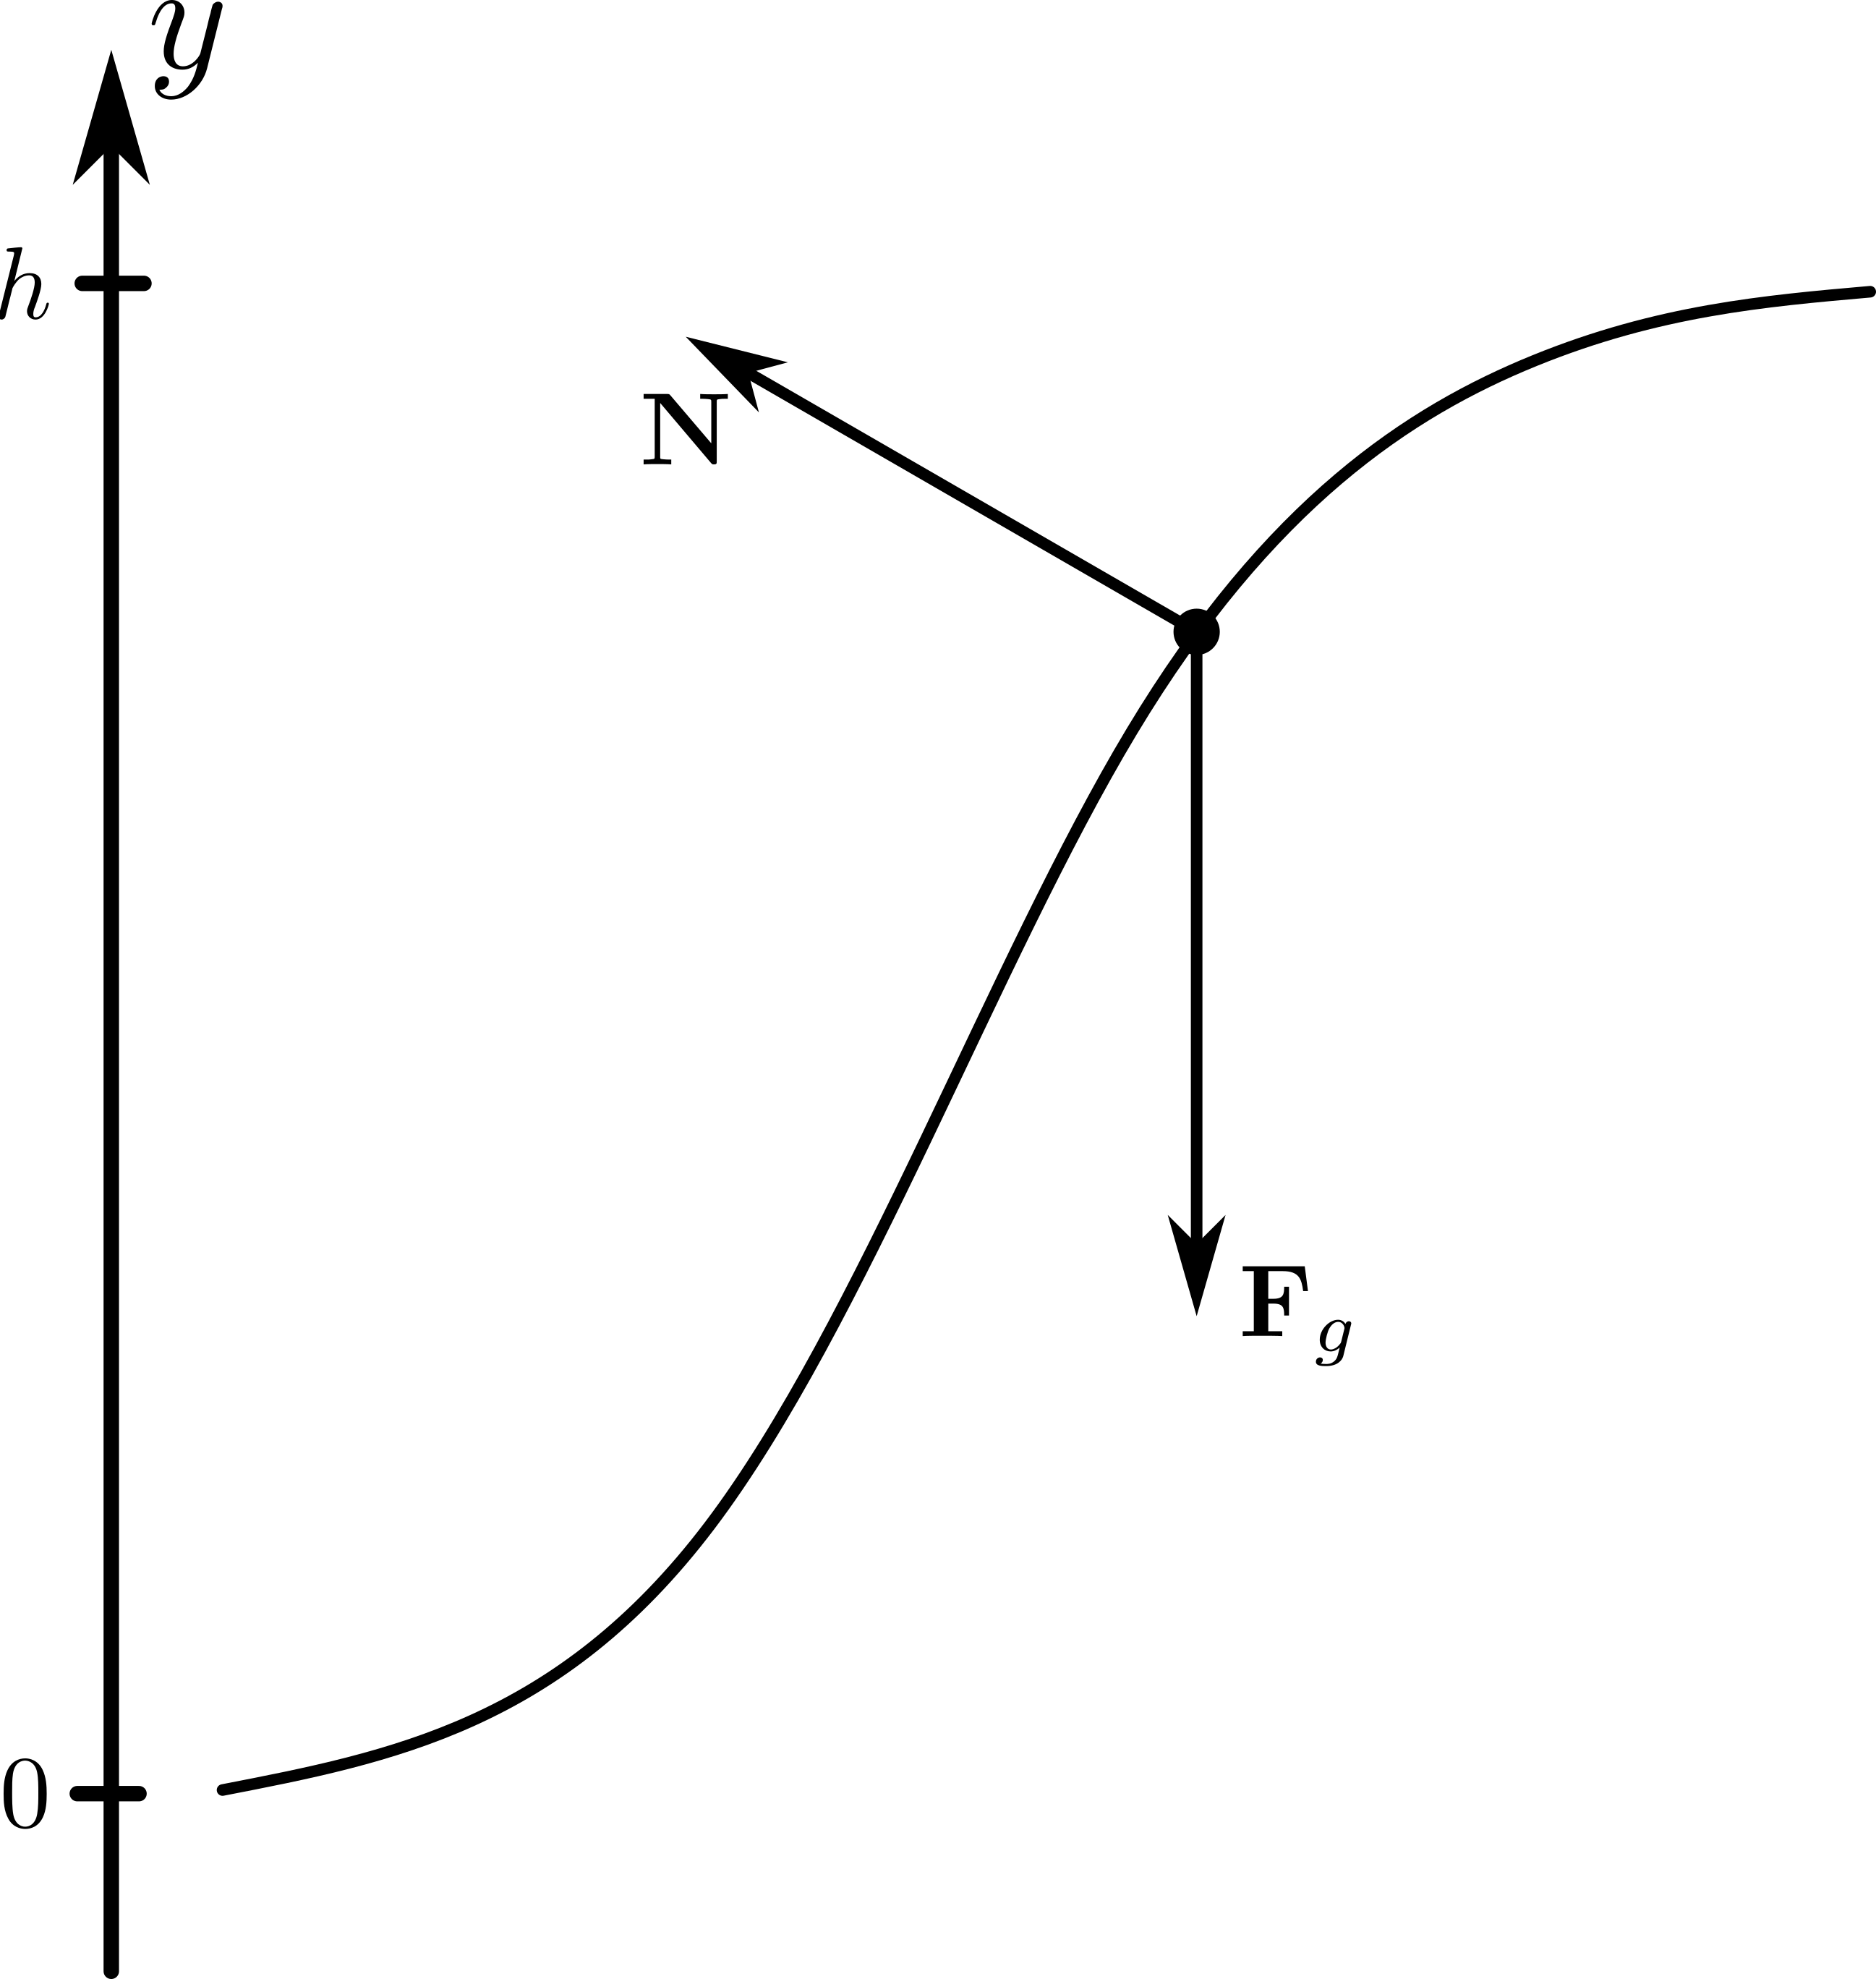
\includegraphics[scale=0.7]{../images/fig4_7.png}
    \caption{A threaded bead on a wire with two forces acting on it; The force of gravity $\vb{F}_g$
    is conservative and the normal force $\vb{N}$ is non-conservative.}
    \label{fig:4_7}
\end{figure}

(c) The bead is initially released from rest at a height $h$. From conservation of energy:
\begin{align}
    E_i &= E_f \\
    \frac{1}{3} m\gamma h^3 &= \frac{1}{2} m v^2 \\
    v &= \sqrt{\frac{2}{3} \gamma h^3}
\end{align}
where $v$ is the speed of the bead at the bottom of the wire.

\paragraph{4.9}
(a) Assuming the force of a one-dimensional spring $F = -kx$ is conservative, potential energy is
\begin{align*}
    U(x) = - \int_0^x F \dd{x'} = \frac{1}{2} kx^2  
\end{align*}
where $x$ is the displacement of the spring from its equilibrium position.

(b) From Newton's second law, the new equilibrium position $x_o$ is found when the spring force and
gravity are equal.
\begin{align*}
    0 = F + F_{g} = -kx_o + m g \implies x_o = \frac{mg}{k}
\end{align*}
When $y = 0$,  $U = 0$. Thus the potential energy is zero at position $x = x_o$:
\begin{align*}
    U(x_o) = \frac{1}{2} k(x_o)^2 - mg(x_o) = 0
\end{align*}
The total potential energy of the system at position $x = y + x_o$ is
\begin{align*}
    U(x) &= U_{sp} + U_{g} = \frac{1}{2} k(y+x_o)^2 - mg(y+x_o) \\
    &= \frac{1}{2} ky^2 + kyx_o - mgy + \frac{1}{2} kx_o^2 - mgx_o
\end{align*}
Since $kyx_o - mgy = 0$ and the last two terms are the potential energy at the new equilibrium
$U(x_o) = 0$, the total potential energy is $U(x) = \frac{1}{2} ky^2$.

\paragraph{4.11}
Finding the partial derivatives of the functions with constants $a,b,c$:

(a) $f(x,y,z) = ax^2 + bxy + cy^2$:
\begin{align*}
    \pdv{f}{x} &= 2ax + by \qquad \pdv{f}{y} = bx + 2cy \qquad \pdv{f}{z} = 0
\end{align*}

(b) $g(x,y,z) = \sin(axyz^2)$:
\begin{align*}
    \pdv{g}{x} &= ayz^2 \cos(axyz^2) \qquad \pdv{g}{y} = axz^2 \cos(axyz^2) 
    \qquad \pdv{g}{z} = 2axyz \cos(axyz^2)
\end{align*}

(c) $h(x,y,z) = ar$ where $r = \sqrt{x^2 + y^2 + z^2}$:
Since 
\begin{equation*}
    \pdv{r}{x_i} = \frac{x_i}{r}
\end{equation*}
The partial derivatives of $h$ are
\begin{align*}
    \pdv{h}{x} &= \frac{ax}{r} \qquad \pdv{h}{y} = \frac{ay}{r} \qquad \pdv{h}{z} = \frac{az}{r}
\end{align*}

\paragraph{4.13}
Calculating the gradient $\grad{f}$ of

(a) $f(x,y,z) = \ln(r) = \ln(\sqrt{x^2 + y^2 + z^2})$:
\begin{align*}
    \pdv{f}{x} &= \frac{x}{r^2} \qquad \pdv{f}{y} = \frac{y}{r^2}
        \qquad \pdv{f}{z} = \frac{z}{r^2} \\
    \grad{f} &= \frac{x}{r^2} \vu{x} + \frac{y}{r^2} \vu{y} + \frac{z}{r^2} \vu{z} 
    = \frac{\vu{r}}{r}
\end{align*}

(b) $f = r^n = (x^2 + y^2 + z^2)^{n/2}$ where $n$ is a constant:
\begin{align*}
    \pdv{f}{x} &= nr^{n-1} \frac{x}{r} = nr^{n-2} x \qquad \pdv{f}{y} = nr^{n-2} y
        \qquad \pdv{f}{z} = nr^{n-2} z \\
    \grad{f} &= nr^{n-2} x \vu{x} + nr^{n-2} y \vu{y} + nr^{n-2} z \vu{z} = nr^{n-1} \vu{r}
\end{align*}

(c) $f = g(r)$ where $g(r)$ is some unspecified function of $r$:
\begin{align*}
    \pdv{f}{x} &= g'(r) \pdv{r}{x} = g'(r) \frac{x}{r} \qquad 
    \pdv{f}{y} = g'(r) \frac{y}{r} \qquad \pdv{f}{z} = g'(r) \frac{z}{r} \\
    \grad{f} &= g'(r) \frac{x}{r} \vu{x} + g'(r) \frac{y}{r} \vu{y} + g'(r) \frac{z}{r} \vu{z}
    = g'(r) \vu{r}
\end{align*}

\paragraph{4.15}
Using the approximate formula for the change in $f$:
\begin{equation*} \tag{4.35}
    \dd{f} = \grad{f} \cdot \dd{\vb{r}}
\end{equation*}
For $f(\vb{r}) = x^2 + 2y^2 + 3z^2$, The approximation of moving from $\vb{r} = (1, 1, 1)$ to
$(1.01, 1.03, 1.05)$:
\begin{align*}
    \dd{f} &= \grad{f} \cdot \dd{\vb{r}} = (2x \vu{x} + 4y \vu{y} + 6z \vu{z}) \cdot 
    (0.01 \vu{x} + 0.03 \vu{y} + 0.05 \vu{z}) \\
    &= 0.02 + 0.12 + 0.30 = 0.44
\end{align*}
The exact change in $f$ is
\begin{align*}
    \Delta f = f(1.01, 1.03, 1.05) - f(1, 1, 1) = 0.4494
\end{align*}

\paragraph{4.17}
A charge $q$ experiences a constant force $\vb{F} = q \vb{E}_o$ where $\vb{E}_o$ is a uniform
electric field. 

(a) The work done by the force from point 1 to 2
\begin{align*}
    W = \int_1^2 \vb{F} \cdot \dd{\vb{r}} = q \vb{E}_o \cdot (\vb{r}_1 - \vb{r}_2)
\end{align*}
which is independent of the path hence it is a conservative force. Thus the potential energy is
\begin{equation*}
    U(\vb{r}) = - W(0 \to \vb{r}) = - q \vb{E}_o \cdot \vb{r}
\end{equation*}

(b) Checking that $\vb{F}$ is derivable from potential energy $U$:
\begin{align*}
    \vb{F} &= - \grad{U} = - \pdv{U}{x} \vu{x} - \pdv{U}{y} \vu{y} - \pdv{U}{z} \vu{z} \\
    &= - \pdv{x}(-q \vb{E}_o \cdot \vb{x}) \vu{x} - \pdv{y}(-q \vb{E}_o \cdot \vb{y}) \vu{y} 
    - \pdv{z}(-q \vb{E}_o \cdot \vb{z}) \vu{z} \\
    &= q \vb{E}_o (\vu{x} + \vu{y} + \vu{z}) = q \vb{E}_o
\end{align*}

\paragraph{4.18}
(a) If the vector $\grad{f}$ is perpendicular to the surface through $r$, then (4.35) becomes
\begin{equation}
    \dd{f} = \grad{f} \cdot \dd{\vb{r}} = 0
\end{equation}
since the dot product of perpendicular vectors is zero. Thus $f$ is constant on the surface.

(b) Choosing a small displacement $\dd{\vb{r}} = \epsilon \vb{u}$:
\begin{equation}
    \dd{f} = \grad{f} \cdot (\epsilon \vb{u}) = \epsilon \grad{f} \cdot \vb{u} 
        = \epsilon \abs{\grad{f}} \abs{\vb{u}} \cos \theta
\end{equation}
the corresponding maximum value of $\dd{f}$ is when $\theta = 0$ where $\vb{u}$ is in the same
direction as $\grad{f}$.

\paragraph{4.19}
(a) For a surface of constant $f$, $f = x^2 + 4y^2$ is an ellipse in the $xy$ plane cenetered at the
origin with semi-major axis $a = \sqrt{f}$ and semi-minor axis $b = \sqrt{f} / 2$. Since $z$ is
unspecified, the surface is an infinitely long elliptical cylinder.

(b) The gradient of $f$ is
\begin{align*}
    \grad{f} = 2x \vu{x} + 8y \vu{y}
\end{align*}
For a surface $f=5$ at the point $(1, 1, 1)$, the gradient is $\grad{f} = 2 \vu{x} + 8 \vu{y}$. From
Problem 4.18, $0 = \grad{f} \cdot \dd{\vb{r}}$ describes that $\grad{f}$ is normal to this surface.
Thus the unit normal vector is
\begin{align*}
    \vu{n} = \frac{\grad{f}}{\abs{\grad{f}}} = \frac{2 \vu{x} + 8 \vu{y}}{\sqrt{68}}
        = \frac{1 \vu{x} + 4 \vu{y}}{\sqrt{17}}
\end{align*}
or $-\vu{n}$ corresponding to the opposite direction. Moving along the direction of $\vb{n}$
maximizes the rate of change of $f$.

\paragraph{4.20}
Finding the curl, $\curl{\vb{F}}$, for the forces:

(a) $\vb{F} = k\vb{r}$
\begin{align*}
    \curl{k\vb{r}} &= \curl(kx \vu{x} + ky \vu{y} + kz \vu{z}) \\
    &= 0 \vu{x} + 0 \vu{y} + 0 \vu{z} = 0
\end{align*}

(b) $\vb{F} = (Ax, By^2, Cz^3)$ where $A,B,C$ are constants:
\begin{align*}
    \curl{(Ax, By^2, Cz^3)} = 0
\end{align*}

(c) $\vb{F} = (Ay^2, Bx, Cz)$:
\begin{align*}
    \curl{(Ay^2, Bx, Cz)} &= 
    \begin{vmatrix}
        \vu{x} & \vu{y} & \vu{z} \\
        \pdv{x} & \pdv{y} & \pdv{z} \\
        Ay^2 & Bx & Cz
    \end{vmatrix} \\
    &= (0) \vu{x} - (0) \vu{y} + (B - 2Ay) \vu{z} = (B - 2Ay) \vu{z}
\end{align*}

\paragraph{4.21}
Given the gravitational force
\begin{align*}
    \vb{F} = - \frac{GmM}{r^2} \vu{r} = - \frac{GmM}{r^3} \vb{r}
\end{align*}
The curl of $\vb{F}$ is
\begin{align*}
    \curl{\vb{F}} &= \curl{\frac{GmM}{r^3} \vb{r}} \\
    &= \frac{GmM}{r^3} \curl{\vb{r}} \\
    &= \frac{GmM}{r^3} \curl{(x \vu{x} + y \vu{y} + z \vu{z})} \\
    &= \frac{GmM}{r^3}
    \begin{vmatrix}
        \vu{x} & \vu{y} & \vu{z} \\
        \pdv{x} & \pdv{y} & \pdv{z} \\
        x & y & z
    \end{vmatrix} \\
    &= \frac{GmM}{r^3} (0 \vu{x} + 0 \vu{y} + 0 \vu{z}) = 0
\end{align*}
Thus the gravitational force is conservative. The potential energy is
\begin{align*}
    U(\vb{r}) = - \int_0^{\vb{r}} \vb{F} \cdot \dd{\vb{r}} = \frac{GmM}{r}
\end{align*}

\paragraph{4.23}
Find which of the following forces are conservative, and for those that are, find the potential and
verify that $\vb{F} = - \grad{U}$:

(a) $\vb{F} = k(x, 2y, 3z)$ where $k$ is a constant. The force is conservative when the curl is zero
\begin{align*}
    \curl{\vb{F}} = k \curl{(x, 2y, 3z)} = 0
\end{align*}
Thus the force is conservative and the potential energy is
\begin{align*}
    U(\vb{r}) = - \int_0^{\vb{r}} \vb{F} \cdot \dd{\vb{r}} = -\frac{1}{2} k(x^2 + 2y^2 + 3z^2)
\end{align*}
Verification of $\vb{F} = - \grad{U}$:
\begin{align*}
    -\grad{U} &= -\quantity(\pdv{U}{x}, \pdv{U}{y}, \pdv{U}{z}) \\
    &= k(x, 2y, 3z) = \vb{F}
\end{align*}

(b) $\vb{F} = k(y, x, 0)$: The curl of $\vb{F}$ is
\begin{align*}
    \curl{\vb{F}} = k \curl{(y, x, 0)} = 0
\end{align*}
Thus the force is conservative and the potential energy is
\begin{align*}
    U(\vb{r}) = - \int_0^{\vb{r}} \vb{F} \cdot \dd{\vb{r}}
    = -\int_0^{\vb{r}} F_x(x, 0) \dd{x'} + F_y(x, y) \dd{y'}
    = -k(xy)
\end{align*}
where the first integral is zero since $F_x = 0$. Differentiating the potential gives
\begin{align*}
    -\grad{U} = -\quantity(\pdv{x}(-kxy), \pdv{y}(-kxy)) = k(y, x) = \vb{F}
\end{align*}

(c) $\vb{F} = k(-y, x, 0)$: The curl of $\vb{F}$ is
\begin{align*}
    \curl{\vb{F}} = k \curl{(-y, x, 0)} = 2k \vu{z}
\end{align*}
Thus the force is not conservative.

\paragraph{4.25}
(a)
\begin{align*}
    \oint_\Gamma \vb{F} \cdot \dd{\vb{r}} &= \int_1^2 \vb{F} \cdot \dd{\vb{r}}
        + \int_2^1 \vb{F} \cdot \dd{\vb{r}} \\
    &= \int_1^1 \vb{F} \cdot \dd{\vb{r}} = 0
\end{align*}

(b)
If $\curl{\vb{F}} = 0$,
\begin{align*}
    \oint_\Gamma \vb{F} \cdot \dd{\vb{r}} &= \int \curl{\vb{F}} \cdot \vu{n} \dd{\vb{A}}
    = 0
\end{align*}

(c)
Integrating $\vb{F}$ around the closed path $\Gamma$:
\begin{align*}
    \oint_\Gamma \vb{F} \cdot \dd{\vb{r}} = &\int_B^{B+b} F_x(x, C, z) \dd{x}
        - \int_B^{B+b} F_x(x, C+c, z) \dd{x} \\
        &+ \int_C^{C+c} F_y(B+b, y, z) \dd{y} - \int_C^{C+c} F_y(B, y, z) \dd{y}
\end{align*}
where the first two terms are the path along the top and bottom of the rectangle and the last two
terms are the path along the left and right sides of the rectangle. Looking at the first two terms,
\begin{align*}
    -\int_B^{B+b} F_x(x, C+c, z) - F_x(x, C, z) \dd{x} 
    = -\int_B^{B+b} \int_C^{C+c} \pdv{F_x(x,y,z)}{y} \dd{y} \dd{x}
    = -\int_S \pdv{F_x}{y} \dd{A}
\end{align*}
The last two terms are
\begin{align*}
    \int_C^{C+c} F_y(B+b, y, z) - F_y(B, y, z) \dd{y} 
    = \int_C^{C+c} \int_B^{B+b} \pdv{F_y(x,y,z)}{x} \dd{x} \dd{y}
    = \int_S \pdv{F_y}{x} \dd{A}
\end{align*}
Hence the integral is
\begin{align*}
    \oint_\Gamma \vb{F} \cdot \dd{\vb{r}} = \int_S \pdv{F_y}{x} - \pdv{F_x}{y} \dd{A}
\end{align*}
where $\curl{\vb{F}} = \pdv{F_y}{x} - \pdv{F_x}{y}$. Thus
\begin{align*}
    \oint_\Gamma \vb{F} \cdot \dd{\vb{r}} = \int_S \curl{\vb{F}} \cdot \vu{n} \dd{A}
\end{align*}

\paragraph{4.27}
From the time-dependent PE for any fixed time $t$
\begin{equation*} \tag{4.48}
    U(\vb{r}, t) = -\int_{\vb{r}_o}^{\vb{r}} \vb{F}(\vb{r}', t) \cdot \dd{\vb{r}'}
\end{equation*}
and the force as a gradient of PE:
\begin{align*}
    -\grad{U}(\vb{r}, t) &= \pdv{U}{r} \int \vb{F}(\vb{r}', t) \cdot \dd{\vb{r}'}
        + \pdv{U}{t} \int \vb{F}(\vb{r}', t) \cdot \dd{\vb{r}'} \\
\end{align*}
Since $t$ is fixed, and by the fundamental theorem of calculus
\begin{align*}
    -\grad{U}(\vb{r}, t) = \vb{F}(\vb{r}, t)
\end{align*}
For closer inspection, the change in $U$ from a small displacement $\dd{\vb{r}}$  and 
\begin{align*}
    \dd{U} = U(\vb{r} + \dd{\vb{r}}, t + \dd{t}) - U(\vb{r}, t)
\end{align*}
rewritten as partial derivatives
\begin{align*}
    \dd{U} = \grad{U} \cdot \dd{\vb{r}} + \pdv{U}{t} \dd{t}
\end{align*}
Given the force is conservative $\vb{F} = -\grad{U}$ and the change in $T$ is defined as
$\dd{T} = \vb{F} \cdot \dd{\vb{r}}$ the work done by the force in the displacement $\dd{\vb{r}}$:
\begin{align*}
    \dd{U} &= -\dd{T} + \pdv{U}{t} \dd{t} \\
    \dd(U + T) &= \pdv{U}{t} \dd{t}
\end{align*}
Hence, the total mechanical energy is conserved only when $\pdv*{U}{t} = 0$ and false otherwise.

\paragraph{4.28}
(a) From conservation of energy, the total mechanical energy is
\begin{align*}
    E = T + U = \frac{1}{2} m \dot{x}^2 + \frac{1}{2} k x^2
\end{align*}
Solving for velocity $\dot{x}$:
\begin{align*}
    \dot{x} = \pm \sqrt{\frac{2}{m} \quantity(E - \frac{1}{2} k x^2)}
\end{align*}
(b) At the spring's max displacement $x_{max} = A$, the kinetic energy is zero hence a total energy
\begin{align*}
    E = U = \frac{1}{2} k A^2
\end{align*}
subbing into the equation for velocity
\begin{align*}
    \dot{x} = \pm \sqrt{\frac{2}{m} \quantity(\frac{1}{2} k A^2 - \frac{1}{2} k x^2)}
    = \pm \sqrt{\frac{k}{m} \quantity(A^2 - x^2)}
\end{align*}
Solving for the time to go from the origin $x=0$ at time $t=0$ to a position $x$ with (4.58):
\begin{align*}
    t = \int_0^x \frac{\dd{x'}}{\dot{x}(x')} 
    = \sqrt{\frac{m}{k}} \int_0^x \frac{\dd{x'}}{\sqrt{(A^2 - x'^2)}}
    = \sqrt{\frac{m}{k}} \arcsin(\frac{x}{A})
\end{align*}
Solving $x$ as a function of $t$:
\begin{align*}
    x = A \sin(\sqrt{\frac{k}{m}} t)
\end{align*}
where the function $\sin(\omega t)$ has a period $T = 2\pi / \omega = 2\pi \sqrt{m/k}$.

\paragraph{4.29}
(a) Figure \ref{fig:4_29} shows the mass moves initially at $t=0$ from $x=0$ to the max displacement
$x=A$ where $E = U = kA^4$. Then it oscillates to and fro from $x=A$ to $x=-A$.
\begin{figure} [ht] 
    \centering
    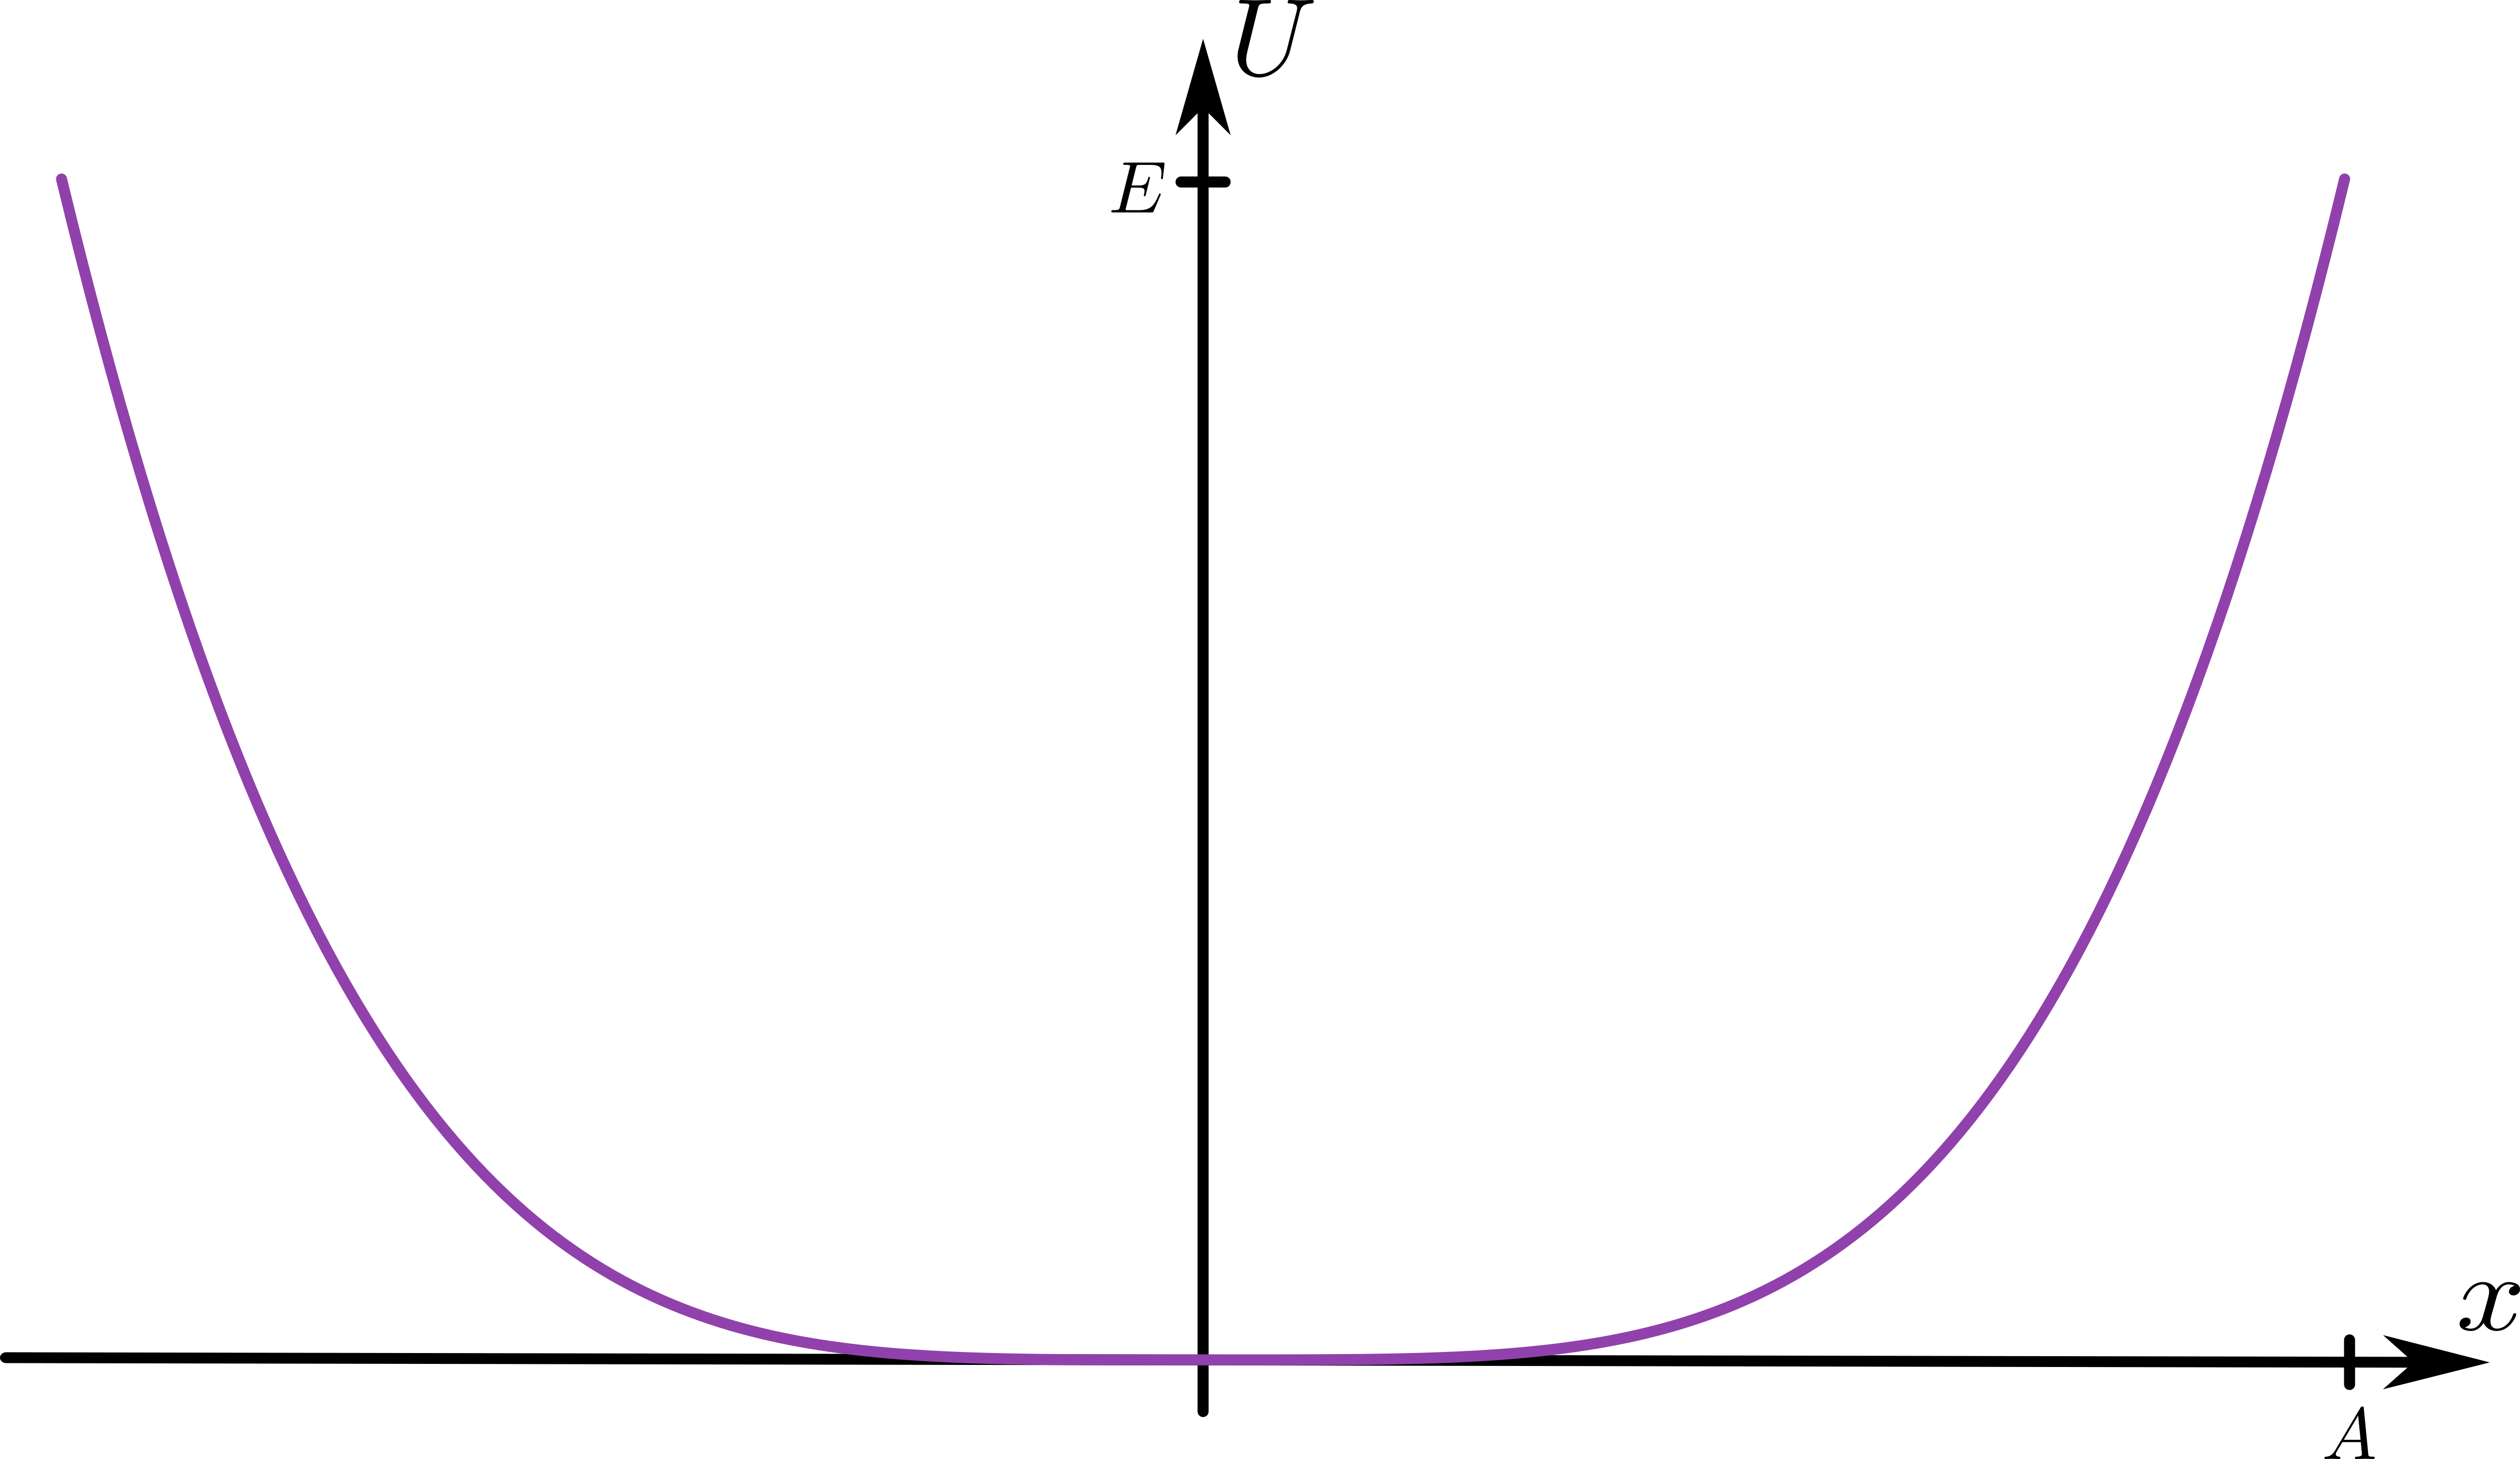
\includegraphics[scale=0.7]{../images/fig4_29.png}
    \caption{A linear system of a mass $m$ with potential energy $U = kx^4$
    force $F_f$.}
    \label{fig:4_29}
\end{figure}

(b) Using (4.58) to find the time it takes to go from $x=0$ to $x=A$:
\begin{align}
    t = \sqrt{\frac{m}{2}} \int_{x_o}^x \frac{\dd{x'}}{E - U(x')}
      = \sqrt{\frac{m}{2k}} \int_0^A \frac{\dd{x'}}{\sqrt{A^4 - x'^4}}
\end{align}
where the period of oscillation $\tau = 4t$ describes the mass moving from $x=0$ to $x=A$ and back
to $x=-A$ and finally back to the initial posistion $x=0$. Hence the period of oscillation
\begin{align*}
    \tau = 4 \sqrt{\frac{m}{2k}} \int_0^A \frac{\dd{x'}}{\sqrt{A^4 - x'^4}}
    = \sqrt{\frac{8m}{k}} \int_0^A \frac{\dd{x'}}{\sqrt{A^4 - x'^4}}
\end{align*}

(c) Changing the variable of integration to $u = x' / A$, $\dd{u} = \dd{x'} / A$: the limits of
integration are $u = 0 \to 1$ and the integrand is $1/\sqrt{1/A^4(1 - x'^4/A^4)}
= 1/(A^2\sqrt{1-u^4})$. Substituting into the integral:
\begin{align*}
    \tau = \frac{1}{A} \sqrt{\frac{8m}{k}} \int_0^1 \frac{\dd{u}}{\sqrt{1 - u^4}}
    = \frac{1}{A} \gamma
\end{align*}
where $\gamma$ is a constant independent of $A$. This clearly shows that that period $\tau$ is
inversely proportional to the amplitude $A$, or simply $\tau \propto 1/A$.

(d) For the case $m = k = A = 1$, the period of oscillation is
\begin{align*}
    \tau = \sqrt{8} \int_0^1 \frac{\dd{u}}{\sqrt{1-u^4}}
\end{align*}
where the integral is numerically evaluated as 1.31 thus $\tau = 3.71$.

\paragraph{4.31}
(a) The total energy $E$ of the two masses in the Atwood machine is
\begin{align*}
    E = T_1 + T_2 + U_1 + U_2
    = \frac{1}{2} m_1 \dot{x}_1^2 + \frac{1}{2} m_2 \dot{x}_2^2 - m_1 g x_1 - m_2 g x_2
\end{align*}
where $x_1 = -x_2 = x$. The total energy is then
\begin{align*}
    E = \frac{1}{2} m_1 \dot{x}^2 + \frac{1}{2} m_2 \dot{x}^2 - m_1 g x + m_2 g x
    = \frac{1}{2} \dot{x}^2 (m_1 + m_2) + (m_2 - m_1) g x
\end{align*}

(b) Differentiating $E$ with respect to time:
\begin{align*}
    \dv{E}{t} = (m_1 + m_2) \dot{x} \ddot{x} + (m_2 - m_1) g \dot{x} = 0
\end{align*}
or rewritten as
\begin{align*}
    (m_1 + m_2) \ddot{x} = (m_1 - m_2) g
\end{align*}
Finding the equation of motion through Newton's second law: the equation of motion for the two
masses are
\begin{align*}
    m_1 \ddot{x}_1 &= m_1 g - T_1 \\
    m_2 \ddot{x}_2 &= T_2 - m_2 g 
\end{align*}
since the tensions $T_1 = T_2 = T$ are equal. Adding the two equations together
\begin{align*}
    (m_1 + m_2) \ddot{x} = (m_1 - m_2) g
\end{align*}
Hence the equation of motions are the same.

\paragraph{4.33}
\begin{figure} [ht]
    \centering
    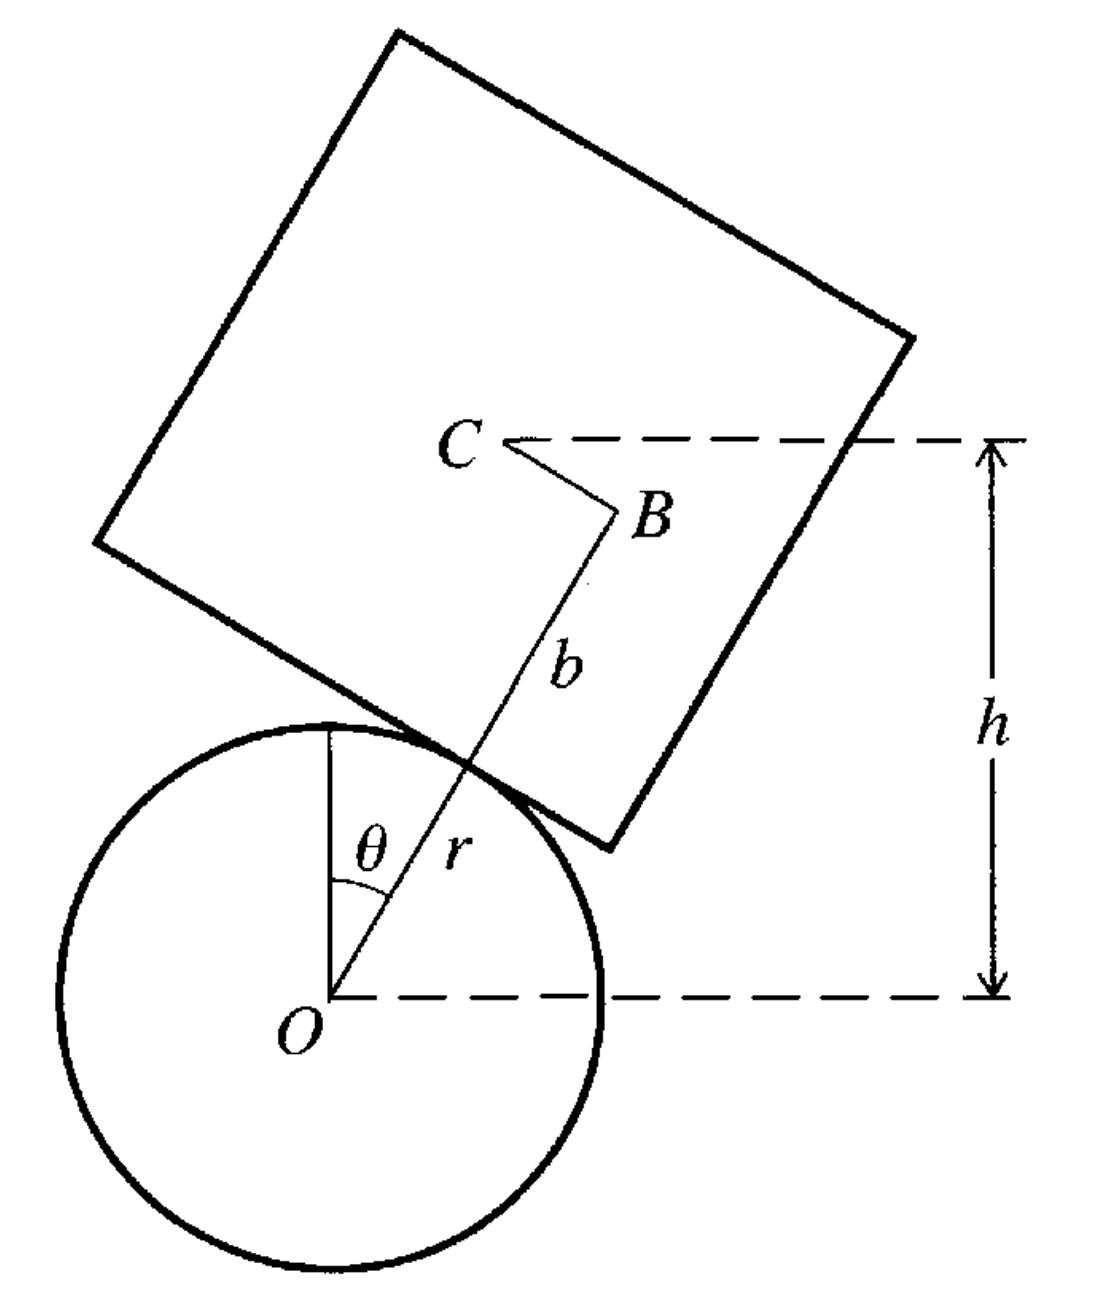
\includegraphics[scale=0.2]{../images/fig4_33.png}
    \captionsetup{width=0.8\textwidth}
    \caption{A cube, of side $2b$ and center C, placed on a fixed cylinder of radius $r$ and center
    $O$. The cube is constrained to roll from side to side without slipping on the cylinder.}
    \label{fig:4_33}
\end{figure}
(a) The forces that constrains the cube to roll without slipping is the frictional force and the
normal force which do no work. With the origin centered at $O$, the potential energy of the cube is
$U = mgh$ where the heigh $h$ is the vertical components of the lines $OB = (r + b)$ and
$BC = r\theta$, the distance the cube rolls from the top of the cylinder:
\begin{align*} \tag{4.59}
    U(\theta) = mgh = mg[(r + b)\cos{\theta} + r\theta\sin\theta]
\end{align*}
(b)
Choosing $r = m = g = 1$, the plot of $U(\theta)$ is shown in Figure \ref{fig:4_33b}.
\begin{figure}[ht]
    \centering
    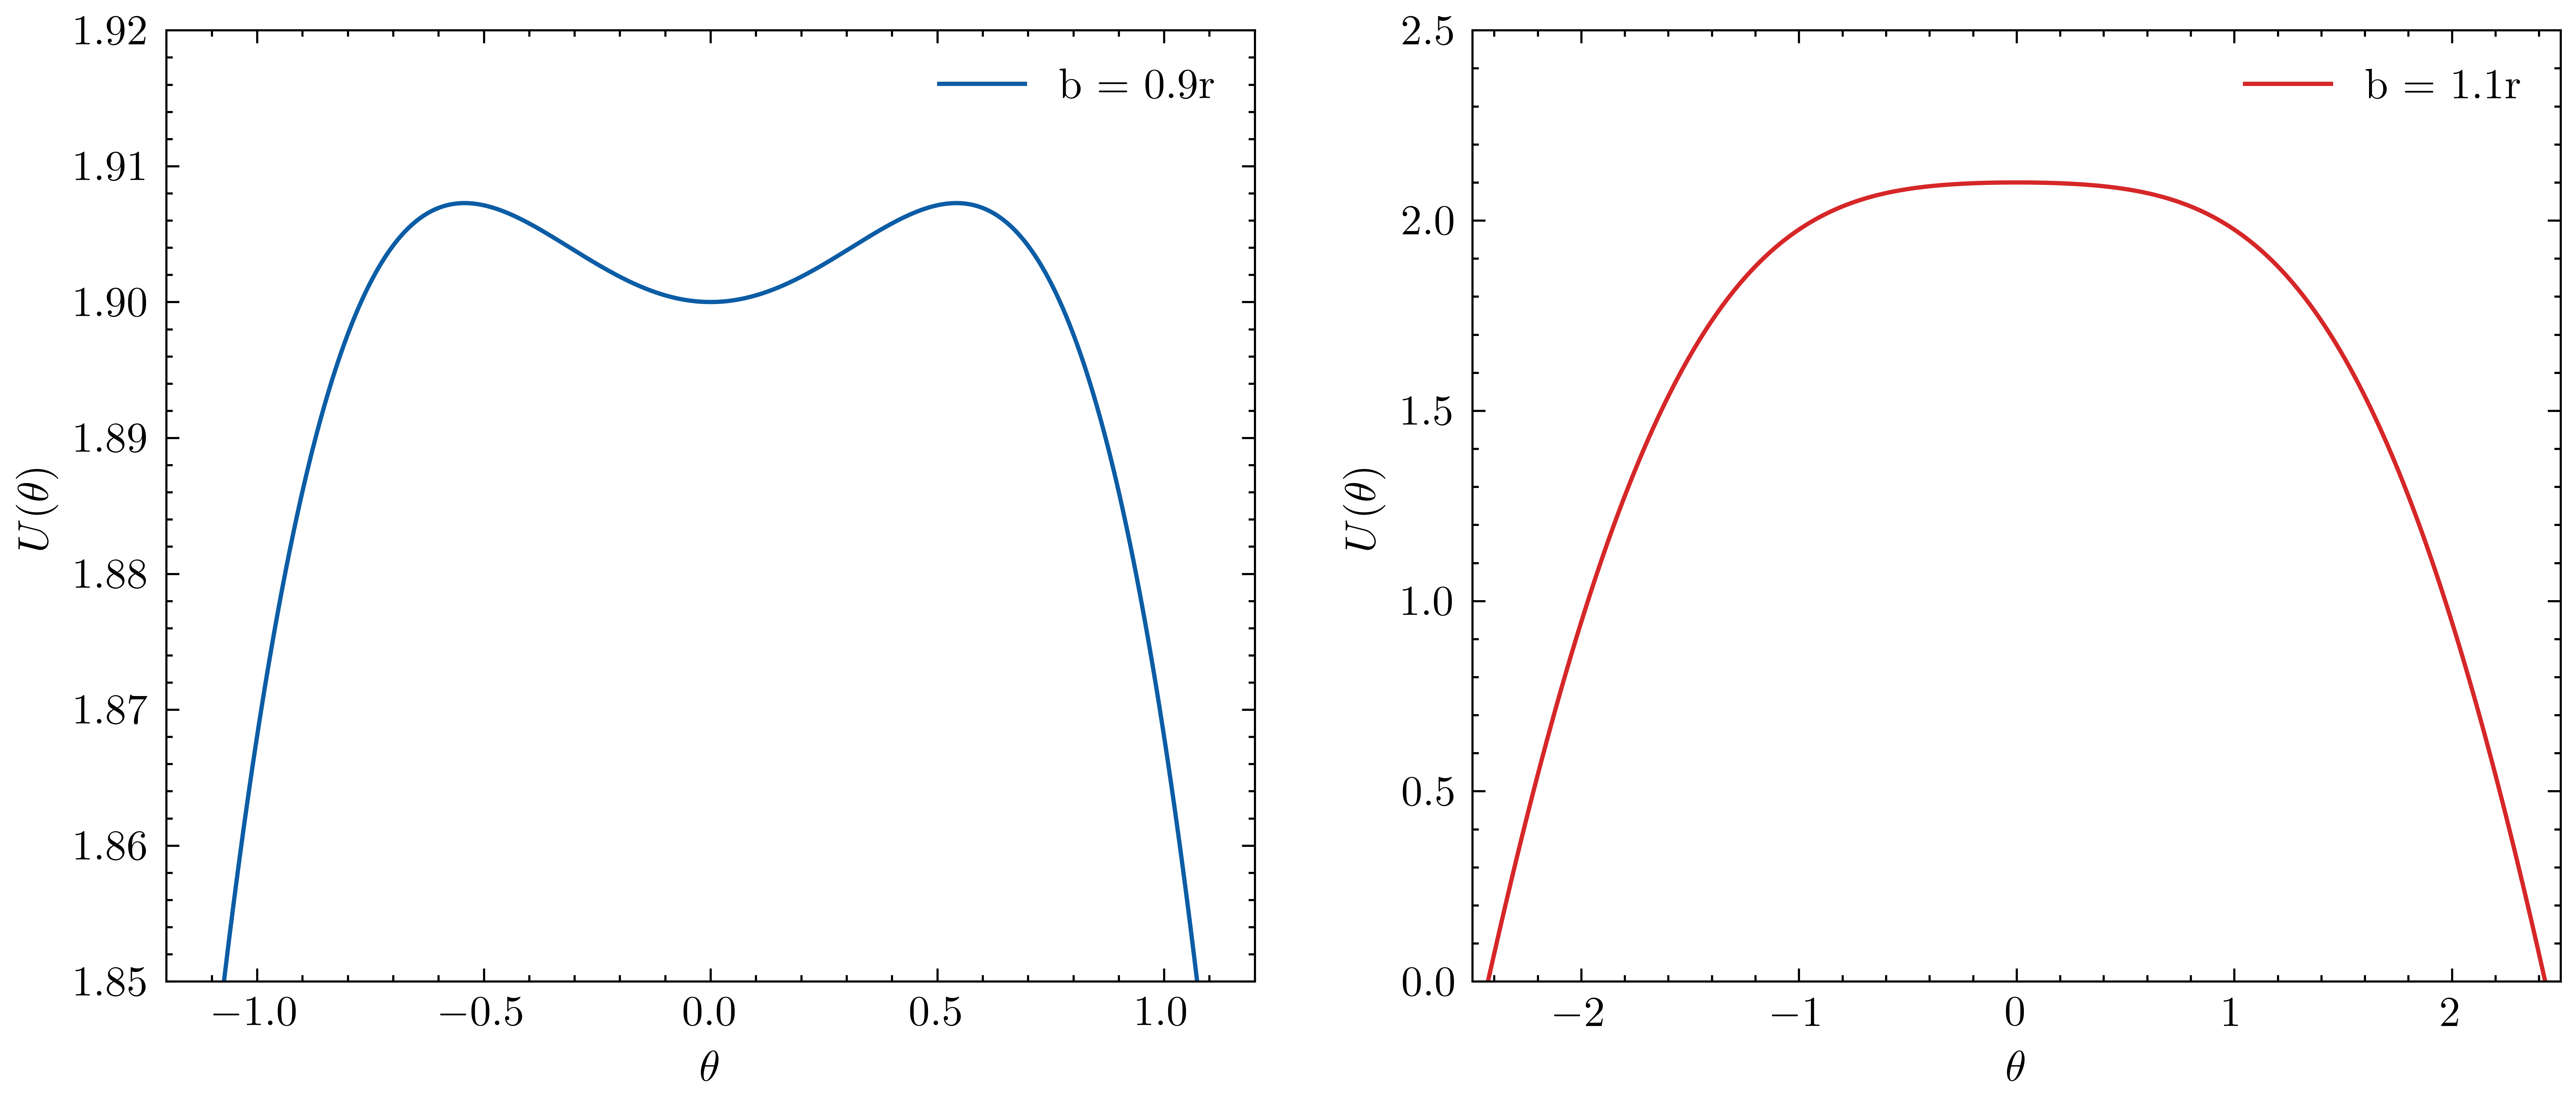
\includegraphics[scale=0.7]{../images/fig4_33b.png}
    \captionsetup{width=0.8\textwidth}
    \caption{The potential energy $U(\theta)$ of the cube as a function of $\theta$.}
    \label{fig:4_33b}
\end{figure}

(c) The equilibrium position $\theta = 0$ is stable for $b = 0.9r$, or when $b < r$, and unstable
for $b = 1.1r$ when $b > r$. For the case $b = 0.9r$, there are two unstable equilibrium points
further away at the two maximum points in Figure \ref{fig:4_33b}.

\paragraph{4.35}
The Atwood machine of Figure \ref{fig:4_33} now has a pulley of radius $R$ and moment of inertia $I$

(a) Given the kinetic energy of the pulley is $T_p = \frac{1}{2} I \omega^2$, the total energy is
\begin{align*}
    E = \frac{1}{2} m_1 \dot{x}_1^2 + \frac{1}{2} m_2 \dot{x}_2^2 + \frac{1}{2} I \omega^2 -
    m_1 g x_1 - m_2 g x_2
\end{align*}
subbing $x_1 = -x_2 = x$ and $\omega = \dot{x}/R$:
\begin{align*}
    E = \frac{1}{2} \dot{x}^2 (m_1 + m_2 + I/R^2) + (m_2 - m_1) g x
\end{align*}
Differentiating $E$ with respect to time:
\begin{align*}
    0 = (m_1 + m_2 + I/R^2) \dot{x} \ddot{x} + (m_2 - m_1) g \dot{x}
\end{align*}
or rewritten as
\begin{align*}
    (m_1 + m_2 + I/R^2) \ddot{x} = (m_1 - m_2) g
\end{align*}
Finding the equation of motion through Newton's second law:
\begin{align*}
    m_1 \ddot{x}_1 &= m_1 g - T_1 \\
    m_2 \ddot{x}_2 &= T_2 - m_2 g \\
    I \dot\omega &= T_1 R - T_2 R
\end{align*}
where $\dot{\omega} = \ddot{x} / R$ and thus $I\ddot{x}/R^2 = T_1 - T_2$. Adding the first two
equations together
\begin{align*}
    (m_1 + m_2) \ddot{x} &= (m_1 - m_2) g - (T_1 - T_2) \\
    (m_1 + m_2) \ddot{x} + (T_1 - T_2) &= (m_1 - m_2) g \\
    (m_1 + m_2 + I/R^2) \ddot{x} &= (m_1 - m_2) g
\end{align*}
Hence the equation of motions are the same.

\paragraph{4.37}
(a) Letting the potential energy $U=mgh$ be zero when $\phi=0$, the height of mass $M$ is $h =
R(1 - \cos\phi)$, and the height of mass $m$ is lowered by the arc length $h = -R\phi$. Therefore,
the total potential energy is
\begin{align*}
    U(\phi) = MgR(1 - \cos\phi) - mgR\phi
\end{align*}

(b) Differentiating $U$ with respect to $\phi$ to find a possible equilibrium position:
\begin{align*}
    \dv{U}{\phi} = MgR\sin\phi - mgR = 0
\end{align*}
Thus the equilibrium position is when $\sin\phi = m/M$. Since the range of $\sin\phi$ is $[-1, 1]$,
the equilibrium position is only possible when $m/M \in [-1, 1]$. Therefore, when $m > M$ there is
no equilibrium position. For the case $m = M$, the equilibrium position is $\phi = \pi/2$. When $m <
M$, there are two equilibrium positions where mass M deviates symmetrically from $\pi/2$ by an angle
$\phi_1$ from both directions. To find stability, we differentiate again:
\begin{align*}
    \dv[2]{U}{\phi} = MgR\cos\phi
\end{align*}
where the second derivative is positive when $\phi < \pi/2$ and is negative when $\phi > \pi/2$
hence the equilibrium position for the case of $m < M$ the lower equilibrium position is stable and
the upper equilibrium position is unstable. For $m = M$, the equilibrium position is unstable since
the second derivative is zero. In terms of torque, the clockwise torque on mass $M$ must be equal
and opposite to the counterclockwise torque on mass $m$ for equilibrium.

(c) Plotting $U(\phi)$ with $g = R = M = 1$ is shown in Figure \ref{fig:4_37}.
\begin{figure}[ht]
    \centering
    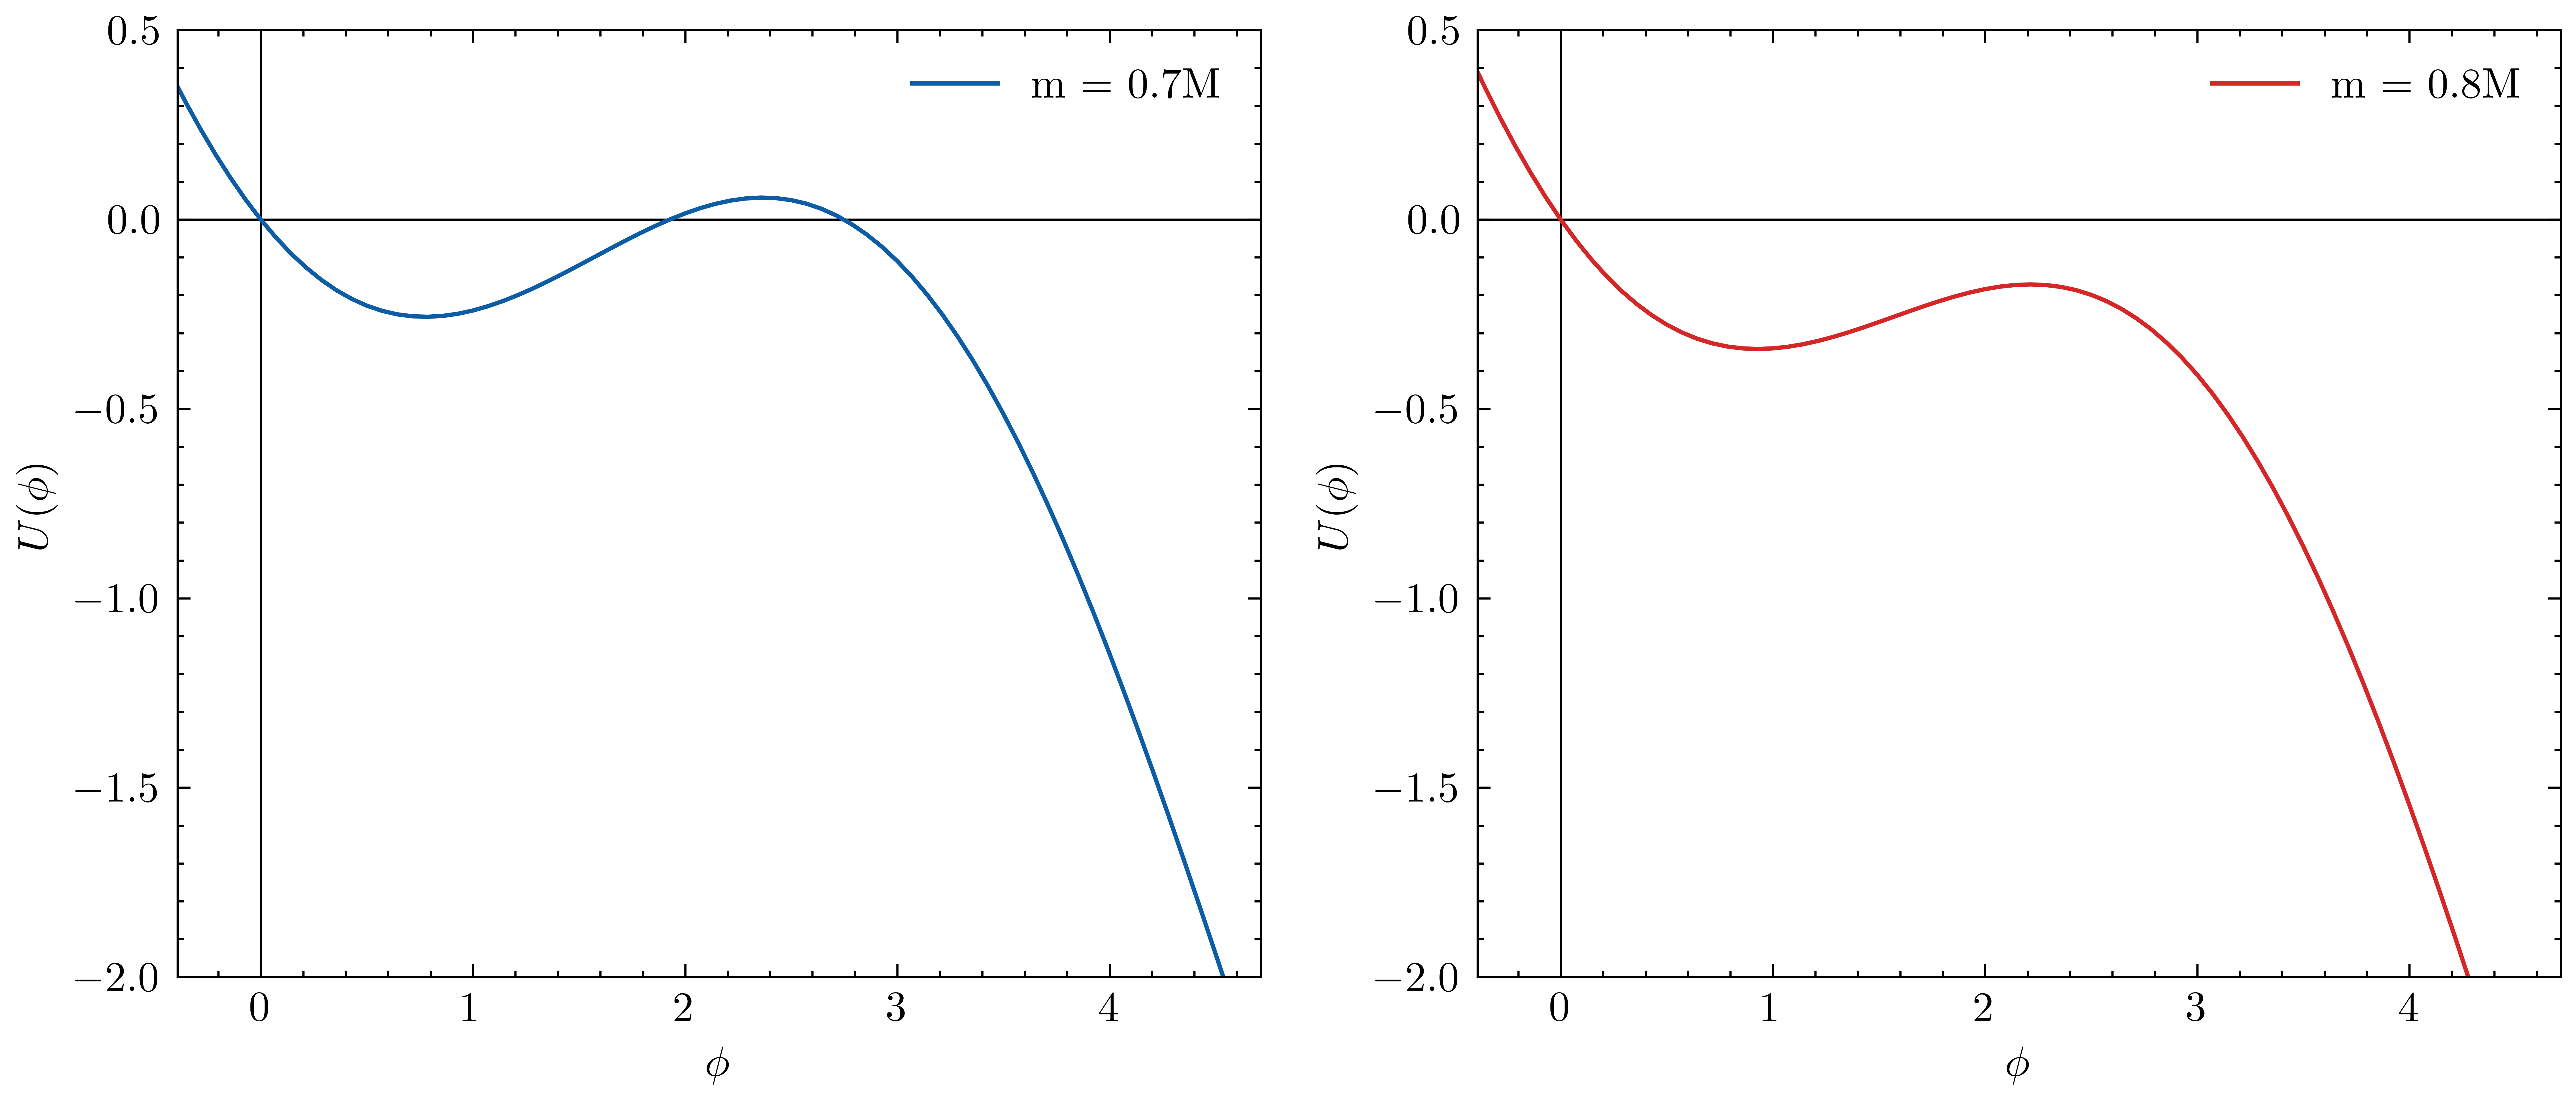
\includegraphics[scale=0.7]{../images/fig4_37.png}
    \captionsetup{width=0.8\textwidth}
    \caption{The potential energy $U(\phi)$ of the system as a function of $\phi$ for the cases
    $m = 0.7M$ and $m = 0.8M$.}
    \label{fig:4_37}
\end{figure}
For the case $m = 0.7M$, when the system is released from rest at $\phi = 0$, the masses will
oscillate about the lower equilibrium position $\phi = \arcsin(0.7) = 0.78$ rad. When $m = 0.8M$,
there is no equilibrium position and the masses will keep rotating ccw.

(d) The critical value of $m/M$ is when the potential energy at the second equilibrium position is
zero, or when the $x$ axis is tangent to the relative maximum of the graph.
\begin{align*}
    0 &= MgR(1 - \cos\phi) - mgR\phi \\
    \cos\phi &= 1 - \frac{m}{M} \phi \\
\end{align*}
combining with $\sin\phi = m/M$:
\begin{align*}
    \cos\phi &= 1 - \phi \sin\phi \\
\end{align*}
The numerical solution is $\phi = 2.33$ rad, so the critical value is $m/M = \sin\phi = 0.72$.

\paragraph{4.39}
(a) Problem 4.28a: The potential energy of a simple pendulum is given by
\begin{equation*}
    U(\phi) = mgl(1 - \cos\phi)
\end{equation*}
The total energy is
\begin{align*}
    E = T + U = \frac{1}{2} ml^2 \dot{\phi}^2 + mgl(1 - \cos\phi)
\end{align*}
where linear velocity $v = l\dot{\phi}$. At the max amplitude $\Phi$, $T = 0$ so the total energy is 
$E = mgl(1 - \cos\Phi)$. $\dot\phi$ as a function of $\phi$ is
\begin{align*}
    \dot{\phi} = \sqrt{\frac{2}{ml^2}} \sqrt{(E - mgl(1 - \cos\phi))}
    = \sqrt{\frac{2g}{l}} \sqrt{(1-\cos\Phi) - (1-\cos\phi)}
\end{align*}
Using the form $t = \int \dd{\phi}/ \dot{\phi}$
\begin{align*}
    t = \sqrt{\frac{l}{2g}} \int_0^\Phi \frac{\dd{\phi}}{\sqrt{(1-\cos\Phi) - (1 - \cos\phi)}}
\end{align*}
since $\tau = 4t$ the period is
\begin{align*}
    \tau = 4 \sqrt{\frac{l}{2g}} \int_0^\Phi \frac{\dd{\phi}}{\sqrt{(1-\cos\Phi) - (1-\cos\phi)}}
\end{align*}
subbing the period for small oscillations $\tau_o = 2\pi \sqrt{l/g}$:
\begin{align*}
    \tau = \tau_o \frac{\sqrt{2}}{\pi} \int_0^\Phi
        \frac{\dd{\phi}}{\sqrt{(1-\cos\Phi) - (1-\cos\phi)}}
\end{align*}
from the half angle identity $1 - \cos(\phi) = 2 \sin^2(\phi/2)$ the square root in the integrand is
\begin{align*}
    \sqrt{(1-\cos\Phi) - (1-\cos\phi)} = \sqrt{2} \sqrt{\sin^2(\Phi/2) - \sin^2(\phi/2)}
\end{align*}
therefore,
\begin{align*}
    \tau = \tau_o \frac{1}{\pi} \int_0^\Phi \frac{\dd{\phi}}{\sqrt{\sin^2(\Phi/2) - \sin^2(\phi/2)}}
\end{align*}
with the substitution $\sin(\phi/2) = Au$ where $A = \sin(\Phi/2)$ and
$\dd{\phi} = \dd{u} 2A/\cos(\phi/2) = 2A/\sqrt{1-A^2 u^2}$ from the relation
\begin{align*}
    \sin^2(\phi/2) = A^2 u^2 = 1 - \cos^2(\phi/2) \to \cos(\phi/2) = \sqrt{1 - A^2 u^2}
\end{align*}
The limits of integration are from $u = 0 \to u = 1$. The square root in the integrand simplifies to
$\sqrt{A^2 - A^2u^2} = A\sqrt{1 - u^2}$, and thus the period is
\begin{align*}
    \tau = \tau_o \frac{2}{\pi} \int_0^1 \frac{\dd{u}}{\sqrt{1-u^2} \sqrt{1-A^2 u^2}}
\end{align*}
and ignoring the last square root for small amplitudes and using the integral
$\int \dd{u}/\sqrt{1-u^2} = \arcsin(u)$:
\begin{align*}
    \tau = \tau_o \frac{2}{\pi} \int_0^1 \frac{\dd{u}}{\sqrt{1-u^2}}
    = \tau_o = 2\pi \sqrt{\frac{l}{g}}
\end{align*}
(c) For a better approximation, using the binomial expansion $1/\sqrt{1-A^2 u^2} \approx
1 + \frac{1}{2} A^2 u^2$:
\begin{align*}
    \tau = \tau_o \frac{2}{\pi} \int_0^1 \frac{1 + \frac{1}{2} A^2 u^2}{\sqrt{1-u^2}} \dd{u}
    = \tau_o + \tau_o \frac{A^2}{\pi} \int_0^1 \frac{u^2}{\sqrt{1-u^2}} \dd{u}
\end{align*}
the integral is evaluated using the substitution $u = \sin(\theta)$ and $\dd{u} = \cos(\theta)
\dd{\theta}$:
\begin{align*}
    \int \frac{u^2}{\sqrt{1-u^2}} \dd{u} = \int \frac{\sin^2(\theta)}{\sqrt{1-\sin^2(\theta)}}
        \cos(\theta) \dd{\theta}
    = \int \sin^2(\theta) \dd{\theta}
\end{align*}
using the half angle identity $\sin^2(\theta) = \frac{1}{2}(1 - \cos(2\theta))$:
\begin{align*}
    \int \sin^2(\theta) \dd{\theta} = \frac{1}{2} \int (1 - \cos(2\theta)) \dd{\theta}
    = \frac{1}{2} \theta - \frac{1}{4} \sin(2\theta)
\end{align*}
subbing back $u = \sin(\theta)$:
\begin{align*}
    \int_0^1 \frac{u^2}{\sqrt{1-u^2}} \dd{u}
    = \frac{1}{2} \arcsin(u) - \frac{1}{4} u \sqrt{1-u^2} \Big|_0^1 = \frac{\pi}{4}
\end{align*}
subbing back to the original equation and using $A = \sin(\Phi/2)$ once more gives
\begin{align*}
    \tau = \tau_o + \tau_o \frac{A^2}{\pi} \frac{\pi}{4} 
    = \tau_o \quantity(1 + \frac{1}{4} \sin^2(\Phi/2))
\end{align*}
Q.E.D

For $\Phi = \ang{45}$, the second term approximation gives $\tau = 1.037\tau_o$ or a 3.7\%
correction compared to the small angle approx $\tau = \tau_o$ and a 0.3\% error compared to the
exact solution $\tau = 1.040\tau_o$.

\paragraph{4.41}
Given $U = kr^n$, taking the derivative with respect to $r$:
\begin{align*}
    F = - \pdv{U}{r} = - kn r^{n-1} = - \frac{n}{r} U
\end{align*}
where the magnitude of force is also equivalent to the centripetal force $F = -mv^2/r$ (the sign
specifies the inward direction). Therefore,
\begin{align*}
    -\frac{mv^2}{r} &= -\frac{n}{r} U \\
    mv^2 &= n U
\end{align*}
Subbing into the KE equation
\begin{align*}
    T = \frac{1}{2} mv^2 = \frac{n}{2} U
\end{align*}

\paragraph{4.43}
(a) For a central and spherically symmetric force
\begin{equation*}
    \vb{F} = f(r) \vu{r} = \frac{f(r)}{r} \vb{r} 
\end{equation*}
Taking the curl of $\vb{F}$:
\begin{align*}
    \curl{\vb{F}} = \det \begin{vmatrix}
        \vu{x} & \vu{y} & \vu{z} \\
        \pdv{x} & \pdv{y} & \pdv{z} \\
        \frac{f(r)x}{r} & \frac{f(r)y}{r} & \frac{f(r)z}{r}
    \end{vmatrix}
\end{align*}
looking at the $x$ component of the curl
\begin{align*}
    (\curl{\vb{F}})_x = \pdv{y} (\frac{f(r)z}{r}) - \pdv{z} (\frac{f(r)y}{r})
\end{align*}
Since $\pdv{{z}}{y} = \pdv{y}{z} = 0$ the equation above is rewritten as
\begin{align*}
    z \pdv{y} (\frac{f(r)}{r}) - y \pdv{z} (\frac{f(r)}{r})
\end{align*}
Next, from the relation
\begin{equation*}
    r = \sqrt{x^2 + y^2 + z^2}
\end{equation*}
and differentiating gives
\begin{align*}
    \pdv{r}{y} = \frac{y}{r}
\end{align*}
and using the chain rule
\begin{equation*}
    \pdv{f(r)}{y} = f'(r)\frac{y}{r}
\end{equation*}
and finally the quotient rule
\begin{align*}
    \pdv{y} (\frac{f(r)}{r}) = \frac{1}{r^2} \quantity( r f'(r) \frac{y}{r} - f(r) \frac{y}{r} )
    = \frac{y}{r^3} \quantity( r f'(r) - f(r) )
\end{align*}
therefore, the $x$ component of the curl is
\begin{align*}
    (\curl{\vb{F}})_x = \frac{zy}{r^3} \quantity( r f'(r) - f(r) ) - \frac{yz}{r^3} \quantity( r
    f'(r) - f(r) ) = 0
\end{align*}
Similarly, the $y$ and $z$ components of the curl are also zero. Hence, a central and spherically
symmetric force is irrotational by $\curl{\vb{F}} = 0$ and thus conservative.

(b) The curl in spherical polar is
\begin{align*}
    \curl{\vb{F}} = \frac{1}{r^2 \sin\theta} \begin{vmatrix}
        \vu{r} & r \vu*{\theta} & r\sin\theta \vu*{\phi} \\
        \pdv{r} & \pdv{\theta} & \pdv{\phi} \\
        (F_r) & r(F_\theta) & r\sin\theta (F_\phi)
    \end{vmatrix}
\end{align*}
where in this case the central force $\vb{F} = f(r) \vu{r}$ implies that the polar and
azimuthal components are $F_\theta = F_\phi = 0$:
\begin{align*}
    \curl{\vb{F}} = \frac{1}{r^2 \sin\theta} \begin{vmatrix}
        \vu{r} & r \vu*{\theta} & r\sin\theta \vu*{\phi} \\
        \pdv{r} & \pdv{\theta} & \pdv{\phi} \\
        f(r) & 0 & 0
    \end{vmatrix}
    = \frac{1}{r^2\sin\theta} \quantity(0 + r \vu*{\theta} \pdv{f(r)}{\phi}
    - r\sin\theta \vu*{\phi} \pdv{f(r)}{\theta})
\end{align*}
where the partial derivatives are
\begin{align*}
    \pdv{r}{\phi} = \pdv{\theta}{\phi} = 0
\end{align*}
therefore
\begin{align*}
    \curl{\vb{F}} = \frac{1}{r^2\sin\theta} \quantity(0 + r \vu*{\theta} f'(r) \pdv{r}{\phi}
    - r\sin\theta \vu*{\phi} f'(r) \pdv{r}{\theta}) = 0
\end{align*}

\paragraph{4.45}
Work done by $\vb{F}(r) = f(\vb{r}) \vu{r}$ from point $A$ to $B$ seperated by an infinitesimal
distance $\dd{r}$ where $r_B = r_A + \dd{r}$: 
\begin{align*}
    W_{AB} = f(\vb{r}) \vu{r} \cdot \dd{\vb{r}}
\end{align*}
The work along both paths are equivalent due to the conservative nature of the force:
\begin{align*}
    W_{ACB} = W_{ADB} \qor W_{AC} + W_{CB} = W_{AD} + W_{DB}
\end{align*}
Since the magnitude of force is perpendicular on the paths $AD$ and $CB$, the work done is zero:
\begin{align*}
    W_{AD} = W_{CB} = 0
\end{align*}
and the work done along the paths $AC$ and $DB$ are equivalent:
\begin{align*}
    W_{AC} &= W_{DB} \\
    f(\vb{r}_A) \dd{r} &= f(\vb{r}_D) \dd{r}
\end{align*}
Since the two position vectors $\vb{r}_A$ and $\vb{r}_D$ have the same magnitude
\begin{align*}
    \abs{\vb{r}_A} = \abs{\vb{r}_D} = r
\end{align*}
the magnitude of the force is the same at both points:
\begin{align*}
    f(\vb{r}_A) = f(\vb{r}_D) = f(r)
\end{align*}
and the force is spherically symmetric.

\paragraph{4.47}
From the conservation of kinetic energy
\begin{align*}
    T_i &= T_f \\
    m_1 v_1^2 + m_2 v_2^2 &= m_1 v_1'^2 + m_2 v_2'^2 \\
    m_1(v_1^2 - v_1'^2) &= m_2(v_2'^2 - v_2^2) \\
\end{align*}
and the conservation of momentum
\begin{align*}
    m_1 v_1 + m_2 v_2 &= m_1 v_1' + m_2 v_2' \\
    m_1(v_1 - v_1') &= m_2(v_2' - v_2)
\end{align*}
dividing the two equations gives
\begin{align*}
    v_1 + v_1' &= v_2 + v_2' \\
    v_1 - v_2 &= -(v_1' - v_2')
\end{align*}

\paragraph{4.49}
Given $\vb{r} = \vb{r}_1 - \vb{r}_2$, the potential energy of the two particle system is
\begin{align*}
    U = \frac{\gamma}{\abs{\vb{r}_1 - \vb{r}_2}} = \frac{\gamma}{\abs{\vb{r}}} = \frac{\gamma}{r}
\end{align*}
and the force on each particle is
\begin{align*}
    \vb{F}_{12} = -\vb{F}_{21} = -\frac{\gamma}{r^3} \vb{r}
\end{align*}
Taking the gradient with respect to $\vb{r}_1$
\begin{align*}
    -\grad_1 U = -\pdv{U}{x_1} \vu{x} - \pdv{U}{y_1} \vu{y} - \pdv{U}{z_1} \vu{z}
\end{align*}
looking at just the $x$ component
\begin{align*}
    -\pdv{U}{x_1} = -\pdv{x_1} \frac{\gamma}{r} = \frac{\gamma}{r^2} \pdv{x_1} r
    = \frac{\gamma}{r^2} \pdv{x_1} \sqrt{(x_1 - x_2)^2 + (y_1 - y_2)^2 + (z_1 - z_2)^2}
\end{align*}
and using the chain rule
\begin{align*}
    \pdv{x_1} \sqrt{(x_1 - x_2)^2 + (y_1 - y_2)^2 + (z_1 - z_2)^2}
    = \frac{x_1 - x_2}{\sqrt{(x_1 - x_2)^2 + (y_1 - y_2)^2 + (z_1 - z_2)^2}}
\end{align*}
therefore
\begin{align*}
    -\pdv{U}{x_1} = \frac{\gamma}{r^3} (x_1 - x_2)
\end{align*}
and similarly for the $y$ and $z$ components
\begin{align*}
    -\pdv{U}{y_1} = \frac{\gamma}{r^3} (y_1 - y_2), \qquad
    -\pdv{U}{z_1} = \frac{\gamma}{r^3} (z_1 - z_2)
\end{align*}
combining the three components
\begin{align*}
    -\grad_1 U = \frac{\gamma}{r^3} \vb{r}
\end{align*}
which is the same as the force on particle 1 $\vb{F}_{12}$. Similarly, the force on particle 2 is
\begin{align*}
    -\grad_2 U = -\frac{\gamma}{r^3} \vb{r} = \vb{F}_{21}
\end{align*}
where the negative sign arises from the partial derivative step.

\paragraph{4.51}
With potential energy defined as $U_{34} = U_{34}(\vb{r}_3 - \vb{r}_4)$, the four particle system
has a potential energy
\begin{align*}
    U = U_{12}(\vb{r}_1 - \vb{r}_2) + U_{13} (\vb{r}_1 - \vb{r}_3) + U_{14} (\vb{r}_1 - \vb{r}_4) \\
    + U_{23} (\vb{r}_2 - \vb{r}_3) + U_{24} (\vb{r}_2 - \vb{r}_4) + U_{34} (\vb{r}_3 - \vb{r}_4) \\
    + U_{1}^{ext} (\vb{r}_1) + U_{2}^{ext} (\vb{r}_2) + U_{3}^{ext} (\vb{r}_3) + U_{4}^{ext}
    (\vb{r}_4)
\end{align*}
The internal forces between a pair of particles are defined as
\begin{align*}
    \vb{F}_{ij} = -\grad_i U_{ij} \qand \vb{F}_{ji} = -\grad_j U_{ij}
\end{align*}
and the external force on particle $\alpha$ depends only on $\vb{r}_\alpha$:
\begin{align*}
    \vb{F}_\alpha^{ext} = -\grad_\alpha U_\alpha^{ext} (\vb{r}_\alpha)
\end{align*} 
when $\grad_3$ acts on $U$ the only the terms with $\vb{r}_3$ are affected:
\begin{align*}
    -\grad_3 U = -\grad_3 (U_{13} + U_{23} + U_{34} + U_3^{ext})
    = \vb{F}_{31} + \vb{F}_{32} + \vb{F}_{34} + \vb{F}_3^{ext}
    = \vb{F}_3^{net}
\end{align*}
where $\vb{F}_3^{net}$ is the net force on particle 3.

\paragraph{4.53} An electron of mass $m$ and charge $-e$ in circular orbit of radius $r$ around a fixed proton of
charge $+e$ where the Coulombic force has magnitude $F = ke^2/r^2$.

(a) The magnitude of force in terms of centripetal acceleration is
\begin{align*}
    F = -\frac{mv^2}{r} = \frac{ke^2}{r^2} \qor mv^2 = \frac{ke^2}{r}
\end{align*}
and the potential energy is
\begin{align*}
    U = -\int F \cdot \dd{r} = -\int \frac{ke^2}{r^2} \dd{r} = -\frac{ke^2}{r}
\end{align*}
the kinetic energy is then
\begin{align*}
    T = \frac{1}{2} mv^2 = \frac{1}{2} \frac{ke^2}{r} = -\frac{1}{2} U
\end{align*}
and the total energy is
\begin{align*}
    E = T + U = -\frac{1}{2} U + U = \frac{1}{2} U
\end{align*}

(b) After electron 1 is knocked out of orbit by electron 2, electron 2 is in orbit of radius $r'$.
The total energy of the system is
\begin{align*}
    E = T_1 + T_2 + U_{12} + U_1 + U_2
\end{align*}
(c) Long before the collision, electron 2 is an infinite distance away from electron 1 and thus
\begin{align*}
    E_i = T_1 + T_2 + U_1 
\end{align*}
Long after the collision
\begin{align*}
    E' = T_1' + T_2' + U_2'
\end{align*}
Since the total energy is conserved
\begin{align*}
    E_i &= E' \\
    T_1 + T_2 + U_1 &= T_1' + T_2' + U_2' \\
    T_1' &= T_1 + T_2 + U_1 - T_2' - U_2' \\
    &= -\frac{1}{2} U_1 + T_2 + U_1 + \frac{1}{2}U_2' - U_2' \\
    &= T_2 + \frac{1}{2} (U_1 - U_2') \\
    &= T_2 + \frac{1}{2} (-ke^2/r + ke^2/r') \\
    T_1' &= T_2 + \frac{1}{2} ke^2 \quantity(\frac{1}{r'} - \frac{1}{r})
\end{align*}
\end{document}